\documentclass{book}
\usepackage{amssymb,amsmath}
\usepackage{polyglossia}
\setmainlanguage{spanish} % Idioma principal
\usepackage{theorem}
\usepackage{times}
\usepackage{array}
\usepackage{graphicx}
\usepackage{hyperref}
\usepackage{multirow}
\usepackage{fancyhdr}
%\usepackage[cp1252]{inputenc}
\usepackage{hhline}
\usepackage{multicol}
\usepackage[a4paper,driver=xetex,top=4.5cm,head=4.5cm, bottom=2cm,%
layouthoffset=0mm, left=2.5cm, right=2.5cm,marginparwidth=0cm]{geometry}
%\usepackage{bm}
%\usepackage{tabular}
\usepackage{fontspec}
 \usepackage[breakable,many]{tcolorbox}
\defaultfontfeatures{Ligatures=TeX}
\usepackage{empheq}
 \setromanfont{Roboto Condensed}
 \usepackage{float}
 \usepackage{mathrsfs} 
%
%
% \renewcommand{\familydefault}{\sfdefault}
%\renewcommand{\familydefault}{\sfdefault}

%%%%%%%%%Estilo de la pagina%%%%%%%%%%%%%%%%%%%%%%%%%%%%%%%%%%%
%%%%%%%%%%%%%%%%%%%%%%%%%%%%%%%%%%%%%%%%%%%%%%%%%%%%%%%%%%%%%%%%%%
% \newcounter{ejer}
% 
% {\theorembodyfont{\normalfont}
% \newtheorem{ejercicio}[ejer]{Ejercicio}}

\newcommand{\rr}{\mathbb{R}}
\newcommand{\qq}{\mathbb{Q}}
\newcommand{\nn}{\mathbb{N}}



\DeclareMathOperator{\atan2}{atan2}
%\DeclareMathOperator{\sen}{sen}
\DeclareMathOperator{\sign}{sign}
\DeclareMathOperator{\sn}{sn}
\DeclareMathOperator{\SO}{SO}
%\DeclareMathOperator{\arcsen}{arcsen}
\DeclareMathOperator{\Or}{O}

\usepackage[framemethod=TikZ]{mdframed}
%%%%%%%%%%%%%%%%%%%%%%%%%%%%%%
%Theorem

%% Ejercicio
\newcounter{ejer} \setcounter{ejer}{0}
\renewcommand{\theejer}{\arabic{ejer}}
\newenvironment{ejer}[2][]{%
\vspace{5pt}
\refstepcounter{ejer}%
\ifstrempty{#1}%
{%
% \mdfsetup{%
% frametitle={%
% \tikz[baseline=(current bounding box.east),outer sep=-0pt]
% \node[anchor=east,rectangle,fill=green!50]
{\noindent\bfseries Ejercicio~\theejer}.}
%
{%
% \mdfsetup{%
% frametitle={%
% \tikz[baseline=(current bounding box.east),outer sep=0pt]
% \node[anchor=east,rectangle,fill=green!50]
{\noindent\bfseries  Ejercicio~\theejer:~#1};}%
%
%\mdfsetup{innertopmargin=10pt,linecolor=green!50,%
%linewidth=2pt,topline=true,%
%frametitleaboveskip=\dimexpr-\ht\strutbox\relax
%}
%\begin{mdframed}[]
\relax%
\label{#2}}{\vspace{5pt}}%\end{mdframed}}

%Theorem
\newcounter{theo}[chapter] \setcounter{theo}{0}
\renewcommand{\thetheo}{\arabic{section}.\arabic{theo}}
\newenvironment{theo}[2][]{%
\refstepcounter{theo}%
\ifstrempty{#1}%
{\mdfsetup{%
frametitle={%
\tikz[baseline=(current bounding box.east),outer sep=0pt]
\node[anchor=east,rectangle,fill=blue!20]
{\strut Teorema~\thetheo};}}
}%
{\mdfsetup{%
frametitle={%
\tikz[baseline=(current bounding box.east),outer sep=0pt]
\node[anchor=east,rectangle,fill=blue!20]
{\strut Teorema~\thetheo:~#1};}}%
}%
\mdfsetup{innertopmargin=10pt,linecolor=blue!20,%
linewidth=2pt,topline=true,%
frametitleaboveskip=\dimexpr-\ht\strutbox\relax
}
\begin{mdframed}[]\relax%
\label{#2}}{\end{mdframed}}
%%%%%%%%%%%%%%%%%%%%%%%%%%%%%%
%Lemma
\newcounter{lem}[chapter] \setcounter{lem}{0}
\renewcommand{\thelem}{\arabic{section}.\arabic{lem}}
\newenvironment{lem}[2][]{%
\refstepcounter{lem}%
\ifstrempty{#1}%
{\mdfsetup{%
frametitle={%
\tikz[baseline=(current bounding box.east),outer sep=0pt]
\node[anchor=east,rectangle,fill=green!20]
{\strut Lemma~\thelem};}}
}%
{\mdfsetup{%
frametitle={%
\tikz[baseline=(current bounding box.east),outer sep=0pt]
\node[anchor=east,rectangle,fill=green!20]
{\strut Lemma~\thelem:~#1};}}%
}%
\mdfsetup{innertopmargin=10pt,linecolor=green!20,%
linewidth=2pt,topline=true,%
frametitleaboveskip=\dimexpr-\ht\strutbox\relax
}
\begin{mdframed}[]\relax%
\label{#2}}{\end{mdframed}}
%%%%%%%%%%%%%%%%%%%%%%%%%%%%%%
%% Definicion
\newcounter{defini}[chapter] \setcounter{defini}{1}
\renewcommand{\thedefini}{\arabic{section}.\arabic{defini}}
\newenvironment{definicion}[2][]{%
\refstepcounter{defini}%
\ifstrempty{#1}%
{\mdfsetup{%
frametitle={%
\tikz[baseline=(current bounding box.east),outer sep=0pt]
\node[anchor=east,rectangle,fill=green!20]
{\strut Definición~\thedefini};}}
}%
{\mdfsetup{%
frametitle={%
\tikz[baseline=(current bounding box.east),outer sep=0pt]
\node[anchor=east,rectangle,fill=green!20]
{\strut Definición~\thedefini:~#1};}}%
}%
\mdfsetup{innertopmargin=10pt,linecolor=green!20,%
linewidth=2pt,topline=true,%
frametitleaboveskip=\dimexpr-\ht\strutbox\relax
}
\begin{mdframed}[]\relax%
\label{#2}}{\end{mdframed}}

%Proof
\newenvironment{prf}{\noindent\emph{Dem.}}{$\square$ \newline\vspace{5pt}}


%Corolario
\newcounter{cor}[chapter] \setcounter{cor}{0}
\renewcommand{\thecor}{\arabic{section}.\arabic{cor}}
\newenvironment{cor}[2][]{%
\refstepcounter{cor}%
\ifstrempty{#1}%
{\mdfsetup{%
frametitle={%
\tikz[baseline=(current bounding box.east),outer sep=0pt]
\node[anchor=east,rectangle,fill=green!20]
{\strut Corolario~\thelem};}}
}%
{\mdfsetup{%
frametitle={%
\tikz[baseline=(current bounding box.east),outer sep=0pt]
\node[anchor=east,rectangle,fill=green!20]
{\strut Corolario~\thelem:~#1};}}%
}%
\mdfsetup{innertopmargin=10pt,linecolor=green!20,%
linewidth=2pt,topline=true,%
frametitleaboveskip=\dimexpr-\ht\strutbox\relax
}
\begin{mdframed}[]\relax%
\label{#2}}{\end{mdframed}}

\tcbset{highlight math style={enhanced,
  colframe=red!60!black,colback=yellow!50!white,arc=4pt,boxrule=1pt,
  drop fuzzy shadow}}
  
  
  
  
  
  
  


\pagestyle{fancyplain}

 \renewcommand{\sectionmark}[1]
                 {\markright{\thesection\ #1}}


% \lhead[\fancyplain{}{\bfseries\thepage}]
%       {\fancyplain{}{\bfseries\rightmark}}
%
 \rhead[\fancyplain{}{\bfseries\leftmark}]{\fancyplain{}{\bfseries}}




 \lhead[\fancyplain{}{ 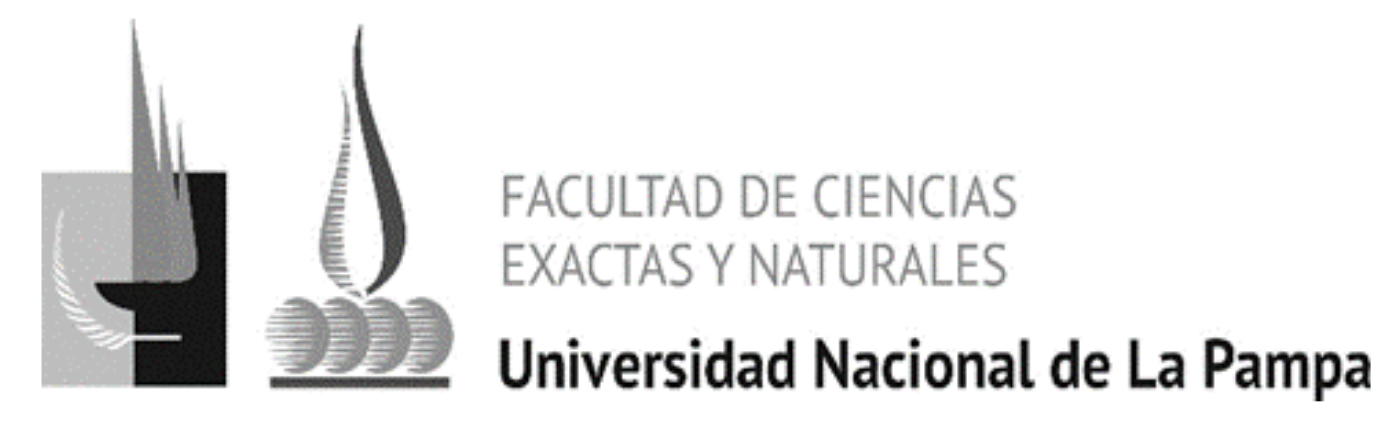
\includegraphics[scale=.3]{EscudoUNLPam.png}}]{\fancyplain{}{ 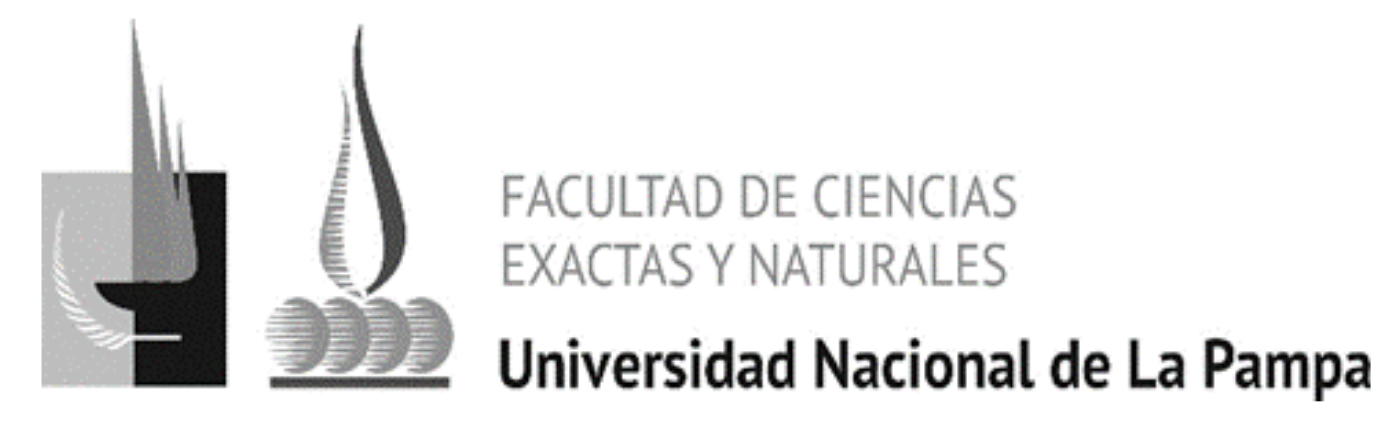
\includegraphics[scale=.3]{EscudoUNLPam.png}}}

\cfoot{}





  
  
  
  
  
  
  
\begin{document}


\hyphenation{excen-tri-ci-dad}


\begin{large}
\begin{bfseries} % \begin{scshape}
        \noindent Depto de Matem\'atica.\\
        Primer Cuatrimestre de 2022\\                                                                                                                                                                                                                                                                                                                                                
        Teoría de la Medida \\
        Práctica 6: Medidas abstractas

%\end{scshape}
\end{bfseries}
\end{large}
\par\noindent\rule{\textwidth}{.5pt}






\begin{ejer}{}
Sea $\mathcal{A}$ una $\sigma$-álgebra.
Probar que si $A_n \in \mathcal{A}$ entonces $\bigcap\limits_{n=1}^{\infty} A_n \in \mathcal{A}$.
\end{ejer}

\begin{ejer}{}
 Mostrar que  $\Sigma$ es $\sigma$-álgebra si y sólo si $\Sigma$ es álgebra y clase monótona.
\end{ejer}


\begin{ejer}{}
 Verificar que $\mathcal{A}=\{(a,+\infty)|a \in \rr\}\cup \{[a,+\infty)|a \in \rr\}$ es clase mónotona pero no 
es álgebra.
\end{ejer}

\begin{ejer}{} Verificar las propiedades de $\sigma$-álgebra y medida.
\begin{enumerate}
\item Sean $X=\rr$, $\mathcal{A}=\mathcal{M}$ la $\sigma$-álgebra de los conjuntos medibles y $\mu$ la medida de Lebesgue.
\item Sean $X=\nn$ y $\{\mu_n\}_{n \in \nn}$ una sucesión con $\mu_n\geq 0$. 
Luego $\mathcal{A}=\mathcal{P}(\nn)$ es $\sigma$-álgebra; y, si $A\in \mathcal{A}$, entonces 
$\mu(A)=\sum\limits_{n \in \mathcal{A}} \mu_n$.
\end{enumerate}
\end{ejer}


\begin{ejer}{} Sea $\mathcal{M}$ la $\sigma$-álgebra de los conjuntos medibles. 
Si $E_n \in \mathcal{M}$ para $n=1,2,3,\ldots$, mutuamente disjuntos,  entonces
\[
\chi_{\bigcup\limits_{n=1}^{\infty}E_n}=\sum\limits_{n=1}^{\infty}\chi_{E_n}
\]
\end{ejer}

\begin{ejer}{} Demostrar que si $\mu$ es una medida sobre una $\sigma$-álgebra,  entonces $\mu(\emptyset)=0$.
\end{ejer}

\begin{ejer}{}
Sean $\mu^*$ medida exterior en $X$ y $\mathcal{A}$ el conjunto de todos los conjuntos 
medibles Carathéodory.
Probar que:
\begin{enumerate}
\item $\emptyset  \in \mathcal{A}$;
\item si $\mu^{*}(E)=0$ entonces $E \in \mathcal{A}$.
\end{enumerate}
\end{ejer}

\begin{ejer}{} Demostrar que:
\begin{enumerate}
\item Si $E_1,E_2,\ldots,E_n \in  \mathcal{A}$ y $E_i\cap E_j=\emptyset$ para $i\neq j$, entonces 
$\mu^{*}(E_1\cup E_2\cup\ldots\cup E_n )=\mu^{*}(E_1)+\mu^{*}(E_2)+\ldots+\mu^{*}(E_n)$.
\item Sea $\mathcal{A}$ un álgebra cualquiera. 

Supongamos que se satisface que 

\textit{
si $E_n \in \mathcal{A}$ para $ n=1,2,\ldots$ son mutuamente disjuntos,  entonces 
$\bigcup\limits_{n=1}^{\infty} E_n\in \mathcal{A}$.}

Probar que $\mathcal{A}$ es $\sigma$-álgebra.
\end{enumerate}
\end{ejer}
	


%¿¿¿¿¿¿¿¿¿¿¿¿¿¿¿¿¿¿¿¿¿¿¿¿¿¿¿¿¿¿¿¿¿¿¿¿¿¿¿


\end{document}
